\documentclass[10pt]{article}
\usepackage[margin=1in]{geometry}\usepackage{graphicx}\usepackage{parskip}
\usepackage{hyperref}\setlength{\parindent}{0pt}
\title{Spatial Degradation of Hepatocyte Zonation\\ Ruler Battery --- Per-Set Report}
\author{Auto-generated}\date{2026-06-21}
\begin{document}\maketitle
\section*{Method (read first)}
Candidate zonation rulers were built, each scored as a per-cell coordinate
(coord $=$ mean\_z(PC) $-$ mean\_z(PP), or a learned projection). \textbf{Ruler quality is judged
ONLY on Paper 2 / healthy-atlas criteria} (8-marker validation gate, healthy PC--PP
anticorrelation, split-half reproducibility). The best healthy ruler is frozen, then transferred
to the Paper 1 disease cohort, where H1/H2/H3 are TEST results --- never used for selection.
Sections below are ordered by healthy-ruler quality (split-half $+\,\max(0,-$anticorr$)$).
H1 = donor-level zonation collapse; H2 = zonal-slope loss; H3 = de-zonation/plasticity coupling.

\paragraph{Selection decision.}\begin{verbatim}
SELECTED set: expanded_curated

Reason: best HEALTHY-ruler quality among primary candidates.
Healthy metrics used (NOT disease collapse):
  validation: 8/8 markers correct
  healthy PC-PP anticorrelation: -0.479 (want strongly negative)
  healthy split-half reproducibility: +0.670
  size: 26 PC + 23 PP

WARNING: selected using Paper 2 / healthy-ruler criteria ONLY, NOT Paper 1 disease effect (disease is the transfer/test cohort, not the tuning cohort).
\end{verbatim}
\clearpage
\section*{unsupervised\_combined \hfill primary\_candidate}
Candidate zonation ruler. \textbf{Genes:} 4769 PC + 3719 PP.
\paragraph{Validation (8-marker healthy gate) \& controls.} Markers correct: 8/8 (PASS). Healthy PC--PP anticorrelation = -0.498 (want strongly negative); split-half reproducibility = +0.720; coherence PC/PP = +0.087/+0.057.
\paragraph{H1 (donor-level collapse, TRANSFER).} coord-spread vs stage rho = -0.514 (perm p = 0.0005); PC--PP anticorr trend rho = +0.625 (perm p = 0.0005).
\paragraph{H2 (zonal slope-loss, held-out).} 100 genes tested; 86\% weaken; median trend rho = -0.258.
\paragraph{H3 (de-zonation $\leftrightarrow$ plasticity, donor-level).} mean rho = -0.010; 24/47 donors $>$0; sign-test p = 1.
\begin{center}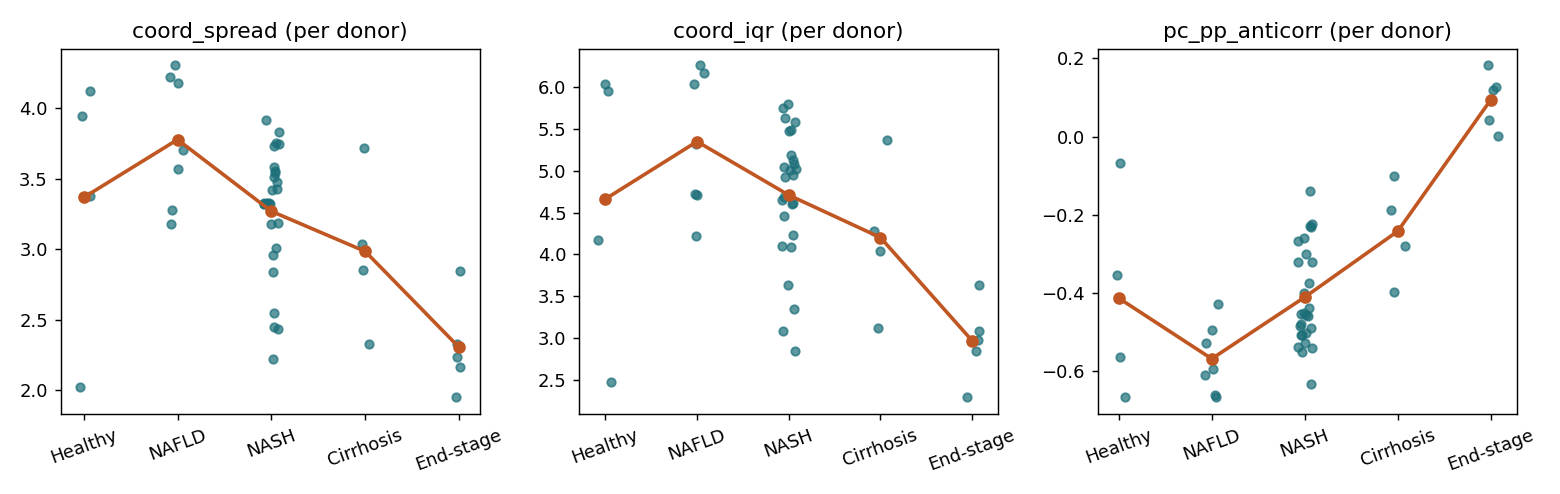
\includegraphics[width=0.92\textwidth]{figures/collapse_unsupervised_combined.png}\end{center}
\clearpage
\section*{unsupervised\_p2 \hfill primary\_candidate}
Candidate zonation ruler. \textbf{Genes:} 5177 PC + 3302 PP.
\paragraph{Validation (8-marker healthy gate) \& controls.} Markers correct: 8/8 (PASS). Healthy PC--PP anticorrelation = -0.471 (want strongly negative); split-half reproducibility = +0.691; coherence PC/PP = +0.076/+0.052.
\paragraph{H1 (donor-level collapse, TRANSFER).} coord-spread vs stage rho = -0.504 (perm p = 0.0005); PC--PP anticorr trend rho = +0.635 (perm p = 0.0005).
\paragraph{H2 (zonal slope-loss, held-out).} 100 genes tested; 83\% weaken; median trend rho = -0.260.
\paragraph{H3 (de-zonation $\leftrightarrow$ plasticity, donor-level).} mean rho = -0.009; 23/47 donors $>$0; sign-test p = 1.
\begin{center}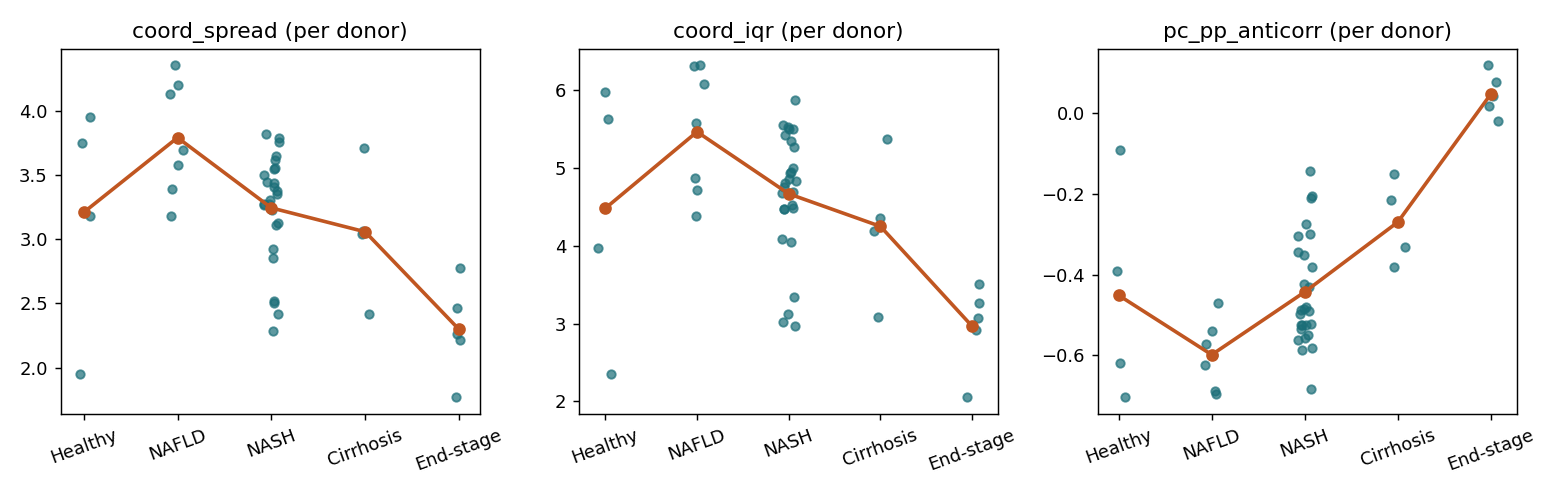
\includegraphics[width=0.92\textwidth]{figures/collapse_unsupervised_p2.png}\end{center}
\clearpage
\section*{expanded\_curated \hfill primary\_candidate}
paper2\_landmark plus curated extra anchors (26+23), de-duplicated. \textbf{Genes:} 26 PC + 23 PP.
\paragraph{Validation (8-marker healthy gate) \& controls.} Markers correct: 8/8 (PASS). Healthy PC--PP anticorrelation = -0.479 (want strongly negative); split-half reproducibility = +0.670; coherence PC/PP = +0.155/+0.065.
\paragraph{H1 (donor-level collapse, TRANSFER).} coord-spread vs stage rho = -0.434 (perm p = 0.003); PC--PP anticorr trend rho = +0.612 (perm p = 0.0005).
\paragraph{H2 (zonal slope-loss, held-out).} 49 genes tested; 90\% weaken; median trend rho = -0.258.
\paragraph{H3 (de-zonation $\leftrightarrow$ plasticity, donor-level).} mean rho = +0.025; 33/47 donors $>$0; sign-test p = 0.0079.
\begin{center}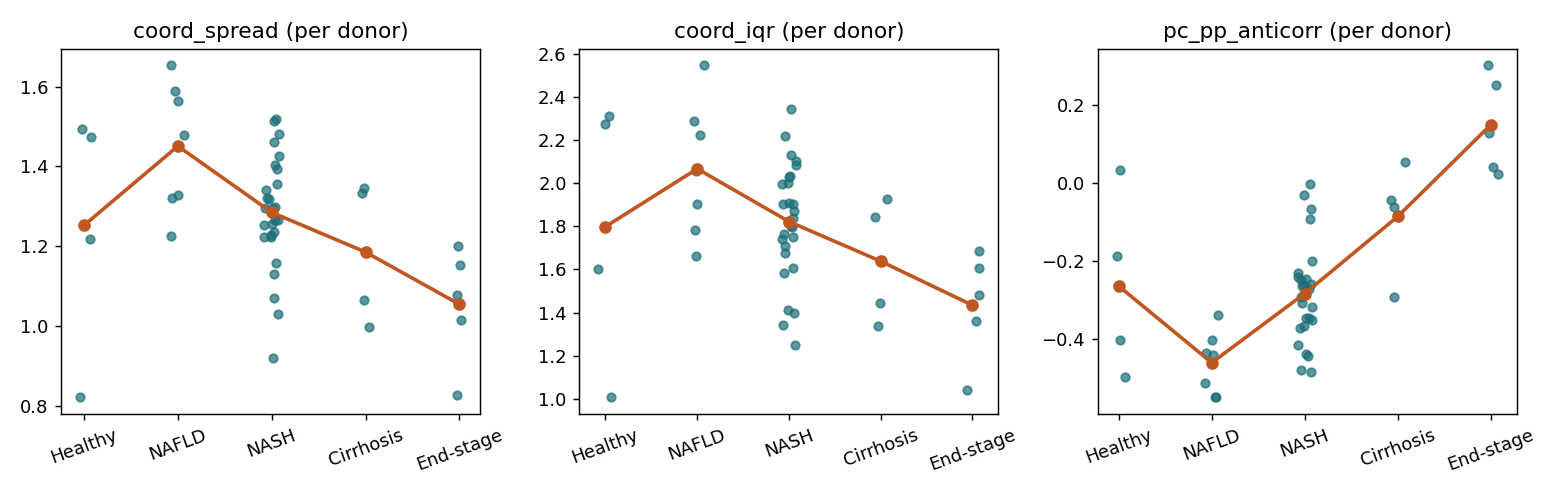
\includegraphics[width=0.92\textwidth]{figures/collapse_expanded_curated.png}\end{center}
\clearpage
\section*{selected\_frozen \hfill primary\_candidate}
The auto-frozen primary ruler (a copy of the best signature set by healthy metrics). \textbf{Genes:} 26 PC + 23 PP.
\paragraph{Validation (8-marker healthy gate) \& controls.} Markers correct: 8/8 (PASS). Healthy PC--PP anticorrelation = -0.479 (want strongly negative); split-half reproducibility = +0.670; coherence PC/PP = +0.155/+0.065.
\paragraph{H1 (donor-level collapse, TRANSFER).} coord-spread vs stage rho = -0.434 (perm p = 0.003); PC--PP anticorr trend rho = +0.612 (perm p = 0.0005).
\paragraph{H2 (zonal slope-loss, held-out).} 49 genes tested; 90\% weaken; median trend rho = -0.258.
\paragraph{H3 (de-zonation $\leftrightarrow$ plasticity, donor-level).} mean rho = +0.025; 33/47 donors $>$0; sign-test p = 0.0079.
\begin{center}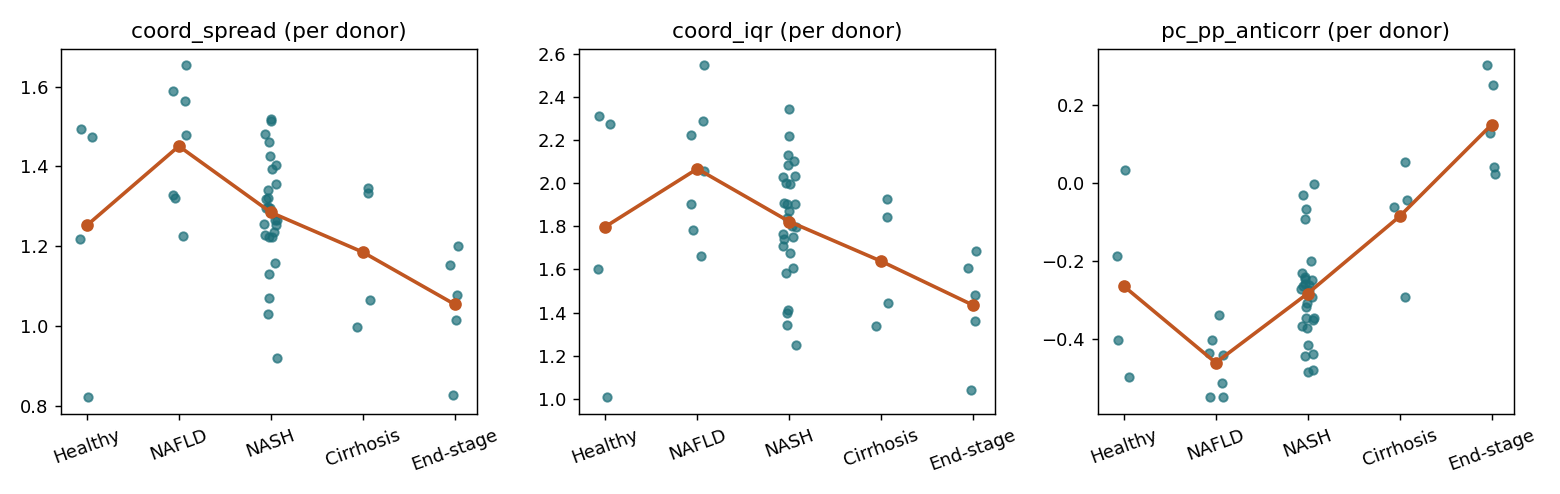
\includegraphics[width=0.92\textwidth]{figures/collapse_selected_frozen.png}\end{center}
\clearpage
\section*{unsupervised\_top100 \hfill primary\_candidate}
The 100+100 strongest +/- loading genes of the unsupervised PCA axis. \textbf{Genes:} 100 PC + 100 PP.
\paragraph{Validation (8-marker healthy gate) \& controls.} Markers correct: 8/8 (PASS). Healthy PC--PP anticorrelation = -0.292 (want strongly negative); split-half reproducibility = +0.821; coherence PC/PP = +0.088/+0.056.
\paragraph{H1 (donor-level collapse, TRANSFER).} coord-spread vs stage rho = -0.608 (perm p = 0.0005); PC--PP anticorr trend rho = +0.613 (perm p = 0.0005).
\paragraph{H2 (zonal slope-loss, held-out).} 200 genes tested; 92\% weaken; median trend rho = -0.324.
\paragraph{H3 (de-zonation $\leftrightarrow$ plasticity, donor-level).} mean rho = +0.031; 36/47 donors $>$0; sign-test p = 0.00035.
\begin{center}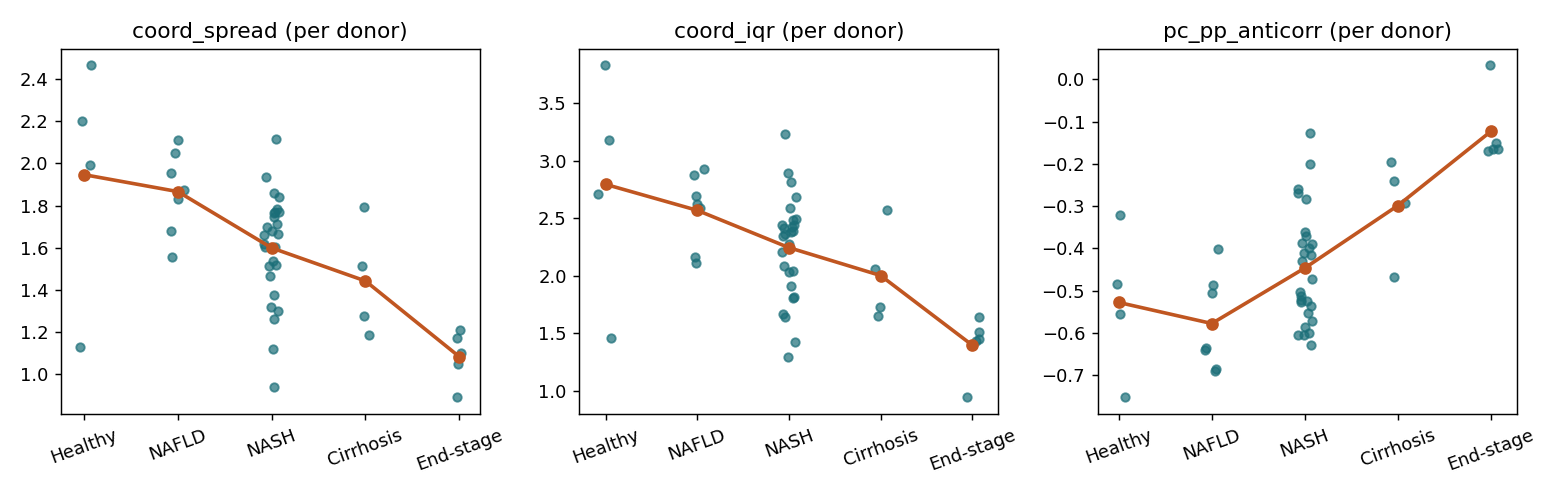
\includegraphics[width=0.92\textwidth]{figures/collapse_unsupervised_top100.png}\end{center}
\clearpage
\section*{unsupervised\_top50 \hfill primary\_candidate}
The 50+50 strongest +/- loading genes of the unsupervised PCA axis, scored as a signature. \textbf{Genes:} 50 PC + 50 PP.
\paragraph{Validation (8-marker healthy gate) \& controls.} Markers correct: 8/8 (PASS). Healthy PC--PP anticorrelation = -0.306 (want strongly negative); split-half reproducibility = +0.785; coherence PC/PP = +0.121/+0.082.
\paragraph{H1 (donor-level collapse, TRANSFER).} coord-spread vs stage rho = -0.617 (perm p = 0.0005); PC--PP anticorr trend rho = +0.607 (perm p = 0.0005).
\paragraph{H2 (zonal slope-loss, held-out).} 100 genes tested; 96\% weaken; median trend rho = -0.372.
\paragraph{H3 (de-zonation $\leftrightarrow$ plasticity, donor-level).} mean rho = +0.027; 38/47 donors $>$0; sign-test p = 2.5e-05.
\begin{center}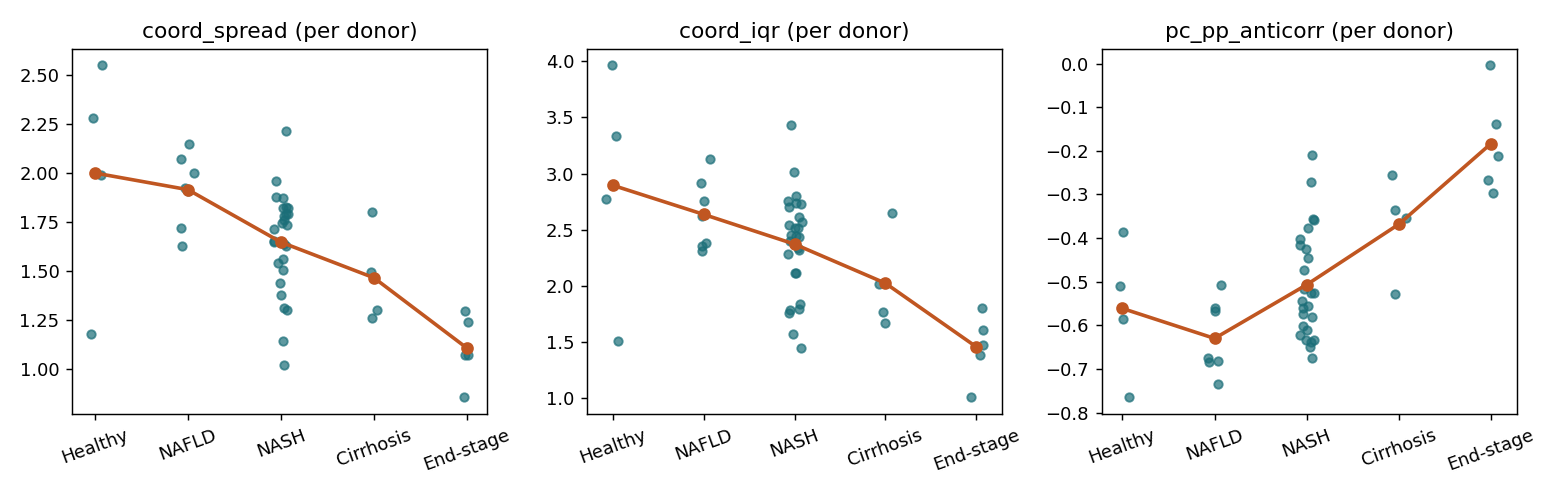
\includegraphics[width=0.92\textwidth]{figures/collapse_unsupervised_top50.png}\end{center}
\clearpage
\section*{unsupervised \hfill primary\_candidate}
Label-free PCA porto-central axis learned on Paper 1 HEALTHY cells (sensitivity version). \textbf{Genes:} 4585 PC + 3903 PP.
\paragraph{Validation (8-marker healthy gate) \& controls.} Markers correct: 7/8 (PASS). Healthy PC--PP anticorrelation = -0.306 (want strongly negative); split-half reproducibility = +0.781; coherence PC/PP = +0.121/+0.082.
\paragraph{H1 (donor-level collapse, TRANSFER).} coord-spread vs stage rho = -0.562 (perm p = 0.0005); PC--PP anticorr trend rho = +0.607 (perm p = 0.0005).
\paragraph{H2 (zonal slope-loss, held-out).} 100 genes tested; 96\% weaken; median trend rho = -0.375.
\paragraph{H3 (de-zonation $\leftrightarrow$ plasticity, donor-level).} mean rho = +0.016; 32/47 donors $>$0; sign-test p = 0.019.
\begin{center}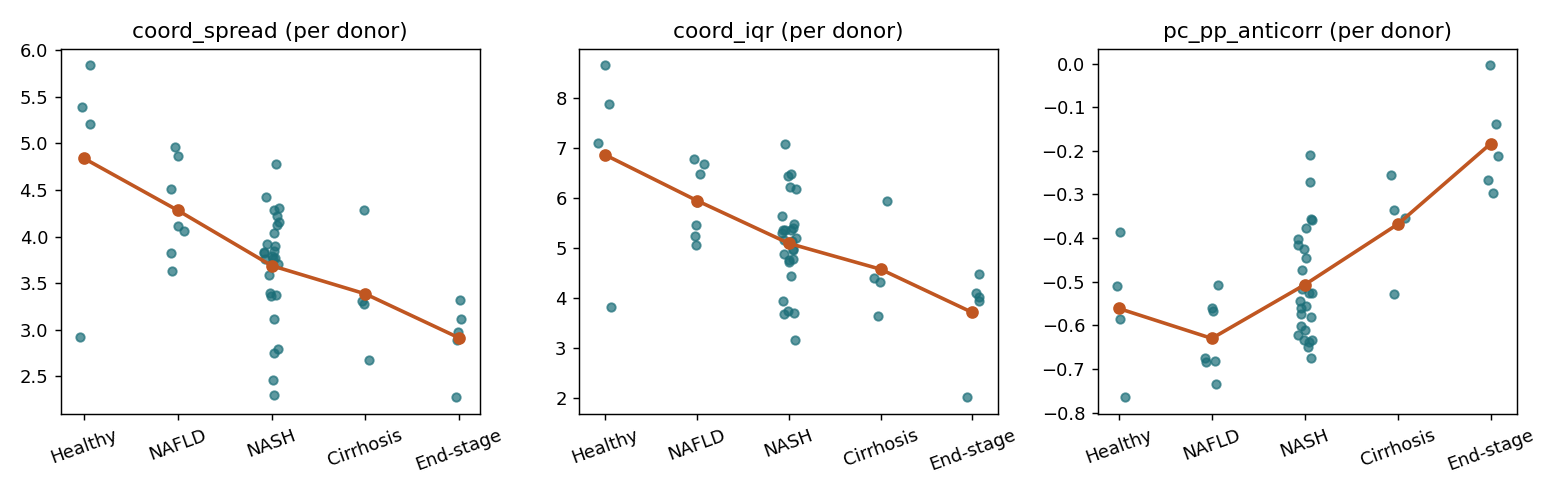
\includegraphics[width=0.92\textwidth]{figures/collapse_unsupervised.png}\end{center}
\clearpage
\section*{paper2\_landmark \hfill primary\_candidate}
Paper 2's exact 20+20 hepatocyte landmark genes (Hepatocyte-\{PC,PP\}-LM.csv), the genes Paper 2 itself uses to assign per-cell snRNA zonation (eta method). \textbf{Genes:} 20 PC + 20 PP.
\paragraph{Validation (8-marker healthy gate) \& controls.} Markers correct: 8/8 (PASS). Healthy PC--PP anticorrelation = -0.455 (want strongly negative); split-half reproducibility = +0.631; coherence PC/PP = +0.156/+0.062.
\paragraph{H1 (donor-level collapse, TRANSFER).} coord-spread vs stage rho = -0.380 (perm p = 0.0085); PC--PP anticorr trend rho = +0.608 (perm p = 0.0005).
\paragraph{H2 (zonal slope-loss, held-out).} 40 genes tested; 78\% weaken; median trend rho = -0.229.
\paragraph{H3 (de-zonation $\leftrightarrow$ plasticity, donor-level).} mean rho = +0.024; 33/47 donors $>$0; sign-test p = 0.0079.
\begin{center}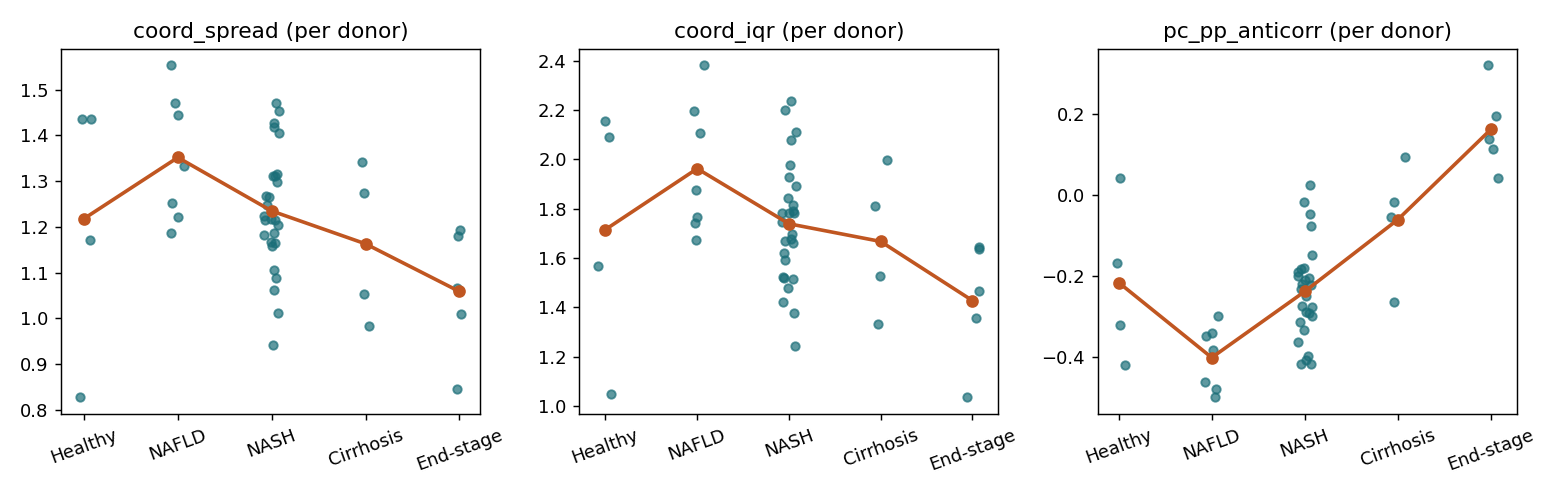
\includegraphics[width=0.92\textwidth]{figures/collapse_paper2_landmark.png}\end{center}
\clearpage
\section*{unsupervised\_top250 \hfill primary\_candidate}
Candidate zonation ruler. \textbf{Genes:} 250 PC + 250 PP.
\paragraph{Validation (8-marker healthy gate) \& controls.} Markers correct: 8/8 (PASS). Healthy PC--PP anticorrelation = -0.227 (want strongly negative); split-half reproducibility = +0.853; coherence PC/PP = +0.047/+0.033.
\paragraph{H1 (donor-level collapse, TRANSFER).} coord-spread vs stage rho = -0.575 (perm p = 0.0005); PC--PP anticorr trend rho = +0.526 (perm p = 0.0005).
\paragraph{H2 (zonal slope-loss, held-out).} 500 genes tested; 81\% weaken; median trend rho = -0.241.
\paragraph{H3 (de-zonation $\leftrightarrow$ plasticity, donor-level).} mean rho = +0.025; 31/47 donors $>$0; sign-test p = 0.04.
\begin{center}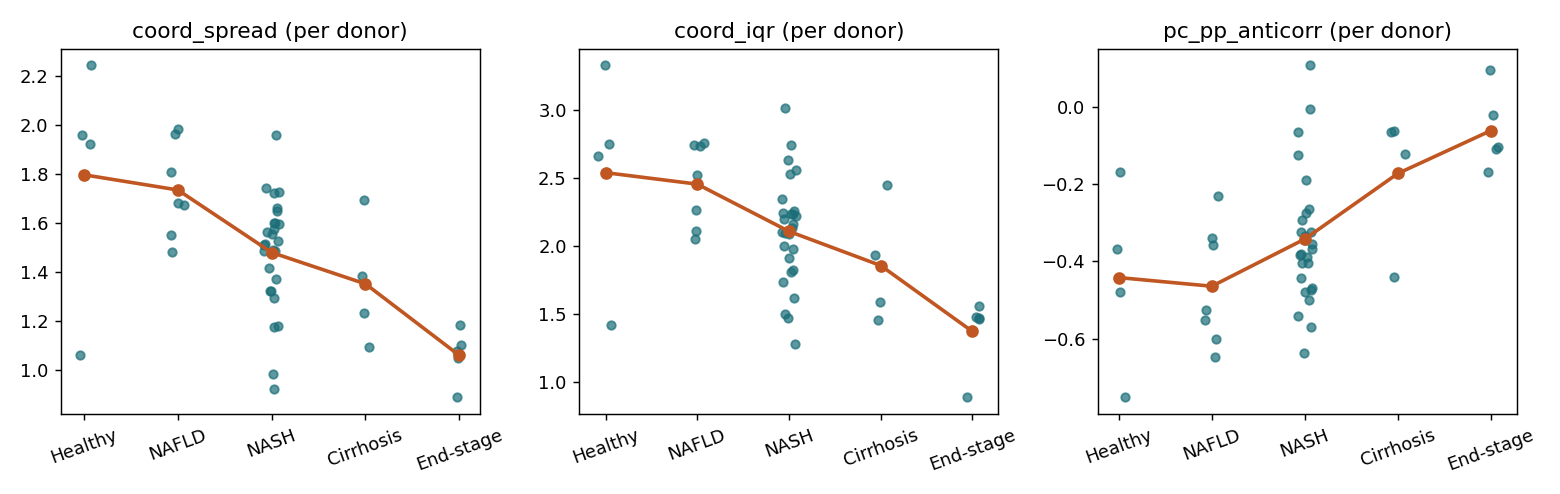
\includegraphics[width=0.92\textwidth]{figures/collapse_unsupervised_top250.png}\end{center}
\clearpage
\section*{paper2\_top50 \hfill primary\_candidate}
Top 50+50 genes by |center-of-mass| among q<0.05 zonated genes (supplementary table 8). \textbf{Genes:} 50 PC + 50 PP.
\paragraph{Validation (8-marker healthy gate) \& controls.} Markers correct: 8/8 (PASS). Healthy PC--PP anticorrelation = -0.404 (want strongly negative); split-half reproducibility = +0.573; coherence PC/PP = +0.051/+0.034.
\paragraph{H1 (donor-level collapse, TRANSFER).} coord-spread vs stage rho = -0.316 (perm p = 0.035); PC--PP anticorr trend rho = +0.564 (perm p = 0.0005).
\paragraph{H2 (zonal slope-loss, held-out).} 88 genes tested; 73\% weaken; median trend rho = -0.204.
\paragraph{H3 (de-zonation $\leftrightarrow$ plasticity, donor-level).} mean rho = +0.010; 33/47 donors $>$0; sign-test p = 0.0079.
\begin{center}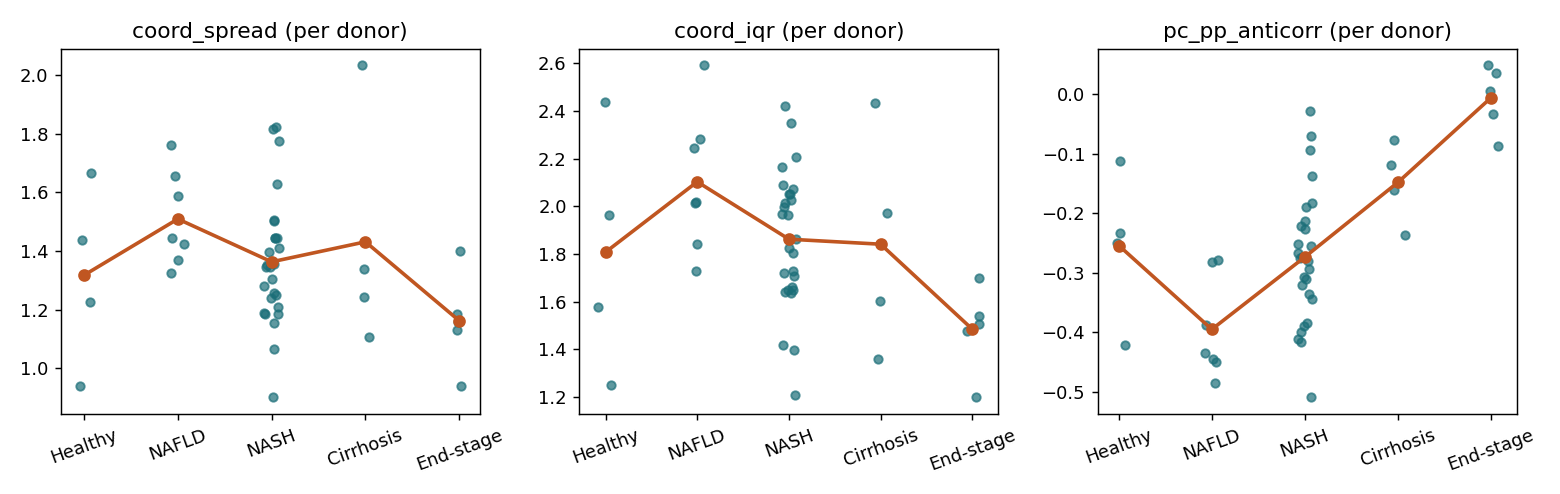
\includegraphics[width=0.92\textwidth]{figures/collapse_paper2_top50.png}\end{center}
\clearpage
\section*{paper2\_top100 \hfill primary\_candidate}
Top 100+100 zonated genes by |center-of-mass|. \textbf{Genes:} 100 PC + 100 PP.
\paragraph{Validation (8-marker healthy gate) \& controls.} Markers correct: 8/8 (PASS). Healthy PC--PP anticorrelation = -0.273 (want strongly negative); split-half reproducibility = +0.563; coherence PC/PP = +0.028/+0.020.
\paragraph{H1 (donor-level collapse, TRANSFER).} coord-spread vs stage rho = -0.284 (perm p = 0.06); PC--PP anticorr trend rho = +0.423 (perm p = 0.003).
\paragraph{H2 (zonal slope-loss, held-out).} 186 genes tested; 59\% weaken; median trend rho = -0.066.
\paragraph{H3 (de-zonation $\leftrightarrow$ plasticity, donor-level).} mean rho = +0.011; 28/47 donors $>$0; sign-test p = 0.24.
\begin{center}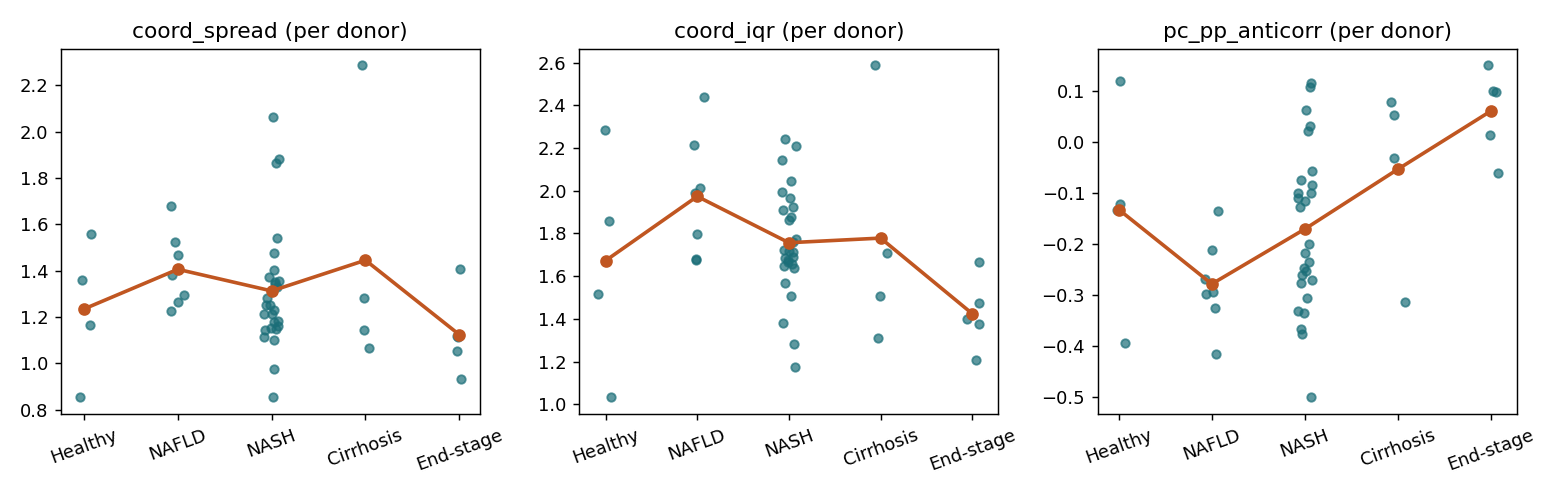
\includegraphics[width=0.92\textwidth]{figures/collapse_paper2_top100.png}\end{center}
\clearpage
\section*{unsupervised\_full \hfill exploratory}
Candidate zonation ruler. \textbf{Genes:} 4585 PC + 3903 PP.
\paragraph{Validation (8-marker healthy gate) \& controls.} Markers correct: 6/8 (PASS). Healthy PC--PP anticorrelation = +0.646 (want strongly negative); split-half reproducibility = +0.831; coherence PC/PP = +0.008/+0.011.
\paragraph{H1 (donor-level collapse, TRANSFER).} coord-spread vs stage rho = -0.421 (perm p = 0.0035); PC--PP anticorr trend rho = +0.196 (perm p = 0.2).
\paragraph{H3 (de-zonation $\leftrightarrow$ plasticity, donor-level).} mean rho = -0.008; 21/47 donors $>$0; sign-test p = 0.56.
\begin{center}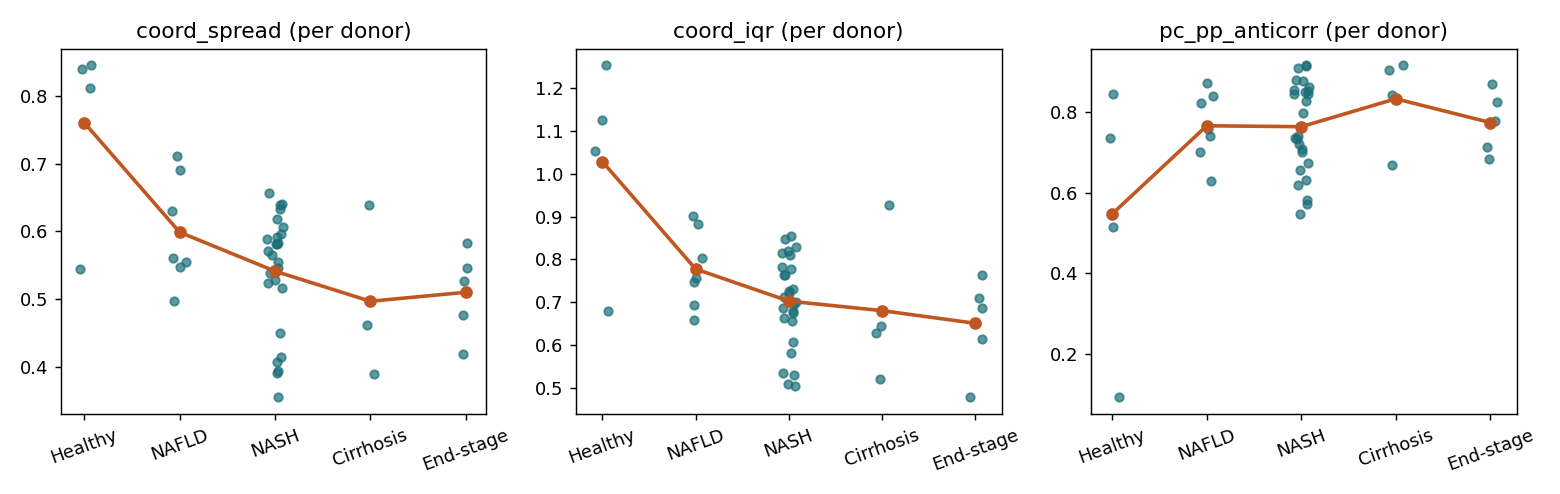
\includegraphics[width=0.92\textwidth]{figures/collapse_unsupervised_full.png}\end{center}
\clearpage
\section*{core\_curated \hfill interpretability\_only}
13+8 hand-curated, highly interpretable canonical anchors (GLUL, CYP2E1, ASS1, HAL, ...). \textbf{Genes:} 13 PC + 8 PP.
\paragraph{Validation (8-marker healthy gate) \& controls.} Markers correct: 8/8 (PASS). Healthy PC--PP anticorrelation = -0.278 (want strongly negative); split-half reproducibility = +0.537; coherence PC/PP = +0.185/+0.104.
\paragraph{H1 (donor-level collapse, TRANSFER).} coord-spread vs stage rho = -0.541 (perm p = 0.0005); PC--PP anticorr trend rho = +0.562 (perm p = 0.0005).
\paragraph{H2 (zonal slope-loss, held-out).} 21 genes tested; 100\% weaken; median trend rho = -0.339.
\paragraph{H3 (de-zonation $\leftrightarrow$ plasticity, donor-level).} mean rho = +0.033; 36/47 donors $>$0; sign-test p = 0.00035.
\begin{center}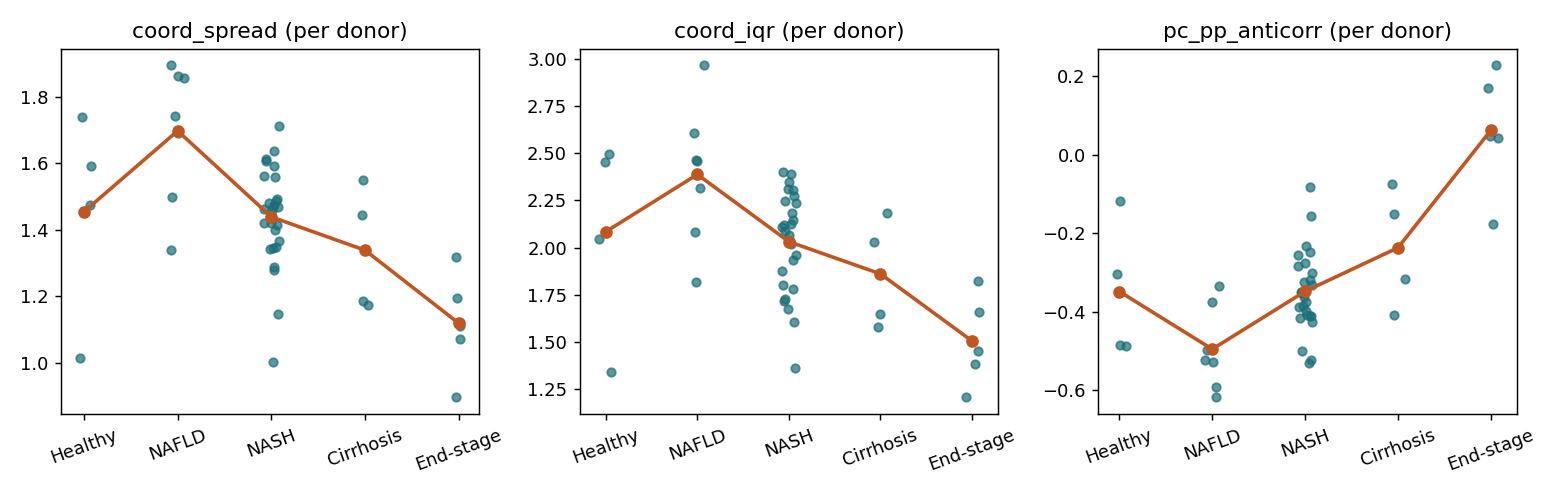
\includegraphics[width=0.92\textwidth]{figures/collapse_core_curated.png}\end{center}
\clearpage
\section*{unsupervised\_lasso \hfill robustness}
Lasso (L1) sparse ruler distilling the Paper-2-trained PCA axis (clean/external training). \textbf{Genes:} 126 PC + 149 PP.
\paragraph{Validation (8-marker healthy gate) \& controls.} Markers correct: 8/8 (PASS). Healthy PC--PP anticorrelation = -0.184 (want strongly negative); split-half reproducibility = +0.629; coherence PC/PP = +0.022/+0.020.
\paragraph{H1 (donor-level collapse, TRANSFER).} coord-spread vs stage rho = -0.505 (perm p = 0.0005); PC--PP anticorr trend rho = +0.602 (perm p = 0.0005).
\paragraph{H2 (zonal slope-loss, held-out).} 275 genes tested; 69\% weaken; median trend rho = -0.144.
\paragraph{H3 (de-zonation $\leftrightarrow$ plasticity, donor-level).} mean rho = -0.017; 22/47 donors $>$0; sign-test p = 0.77.
\begin{center}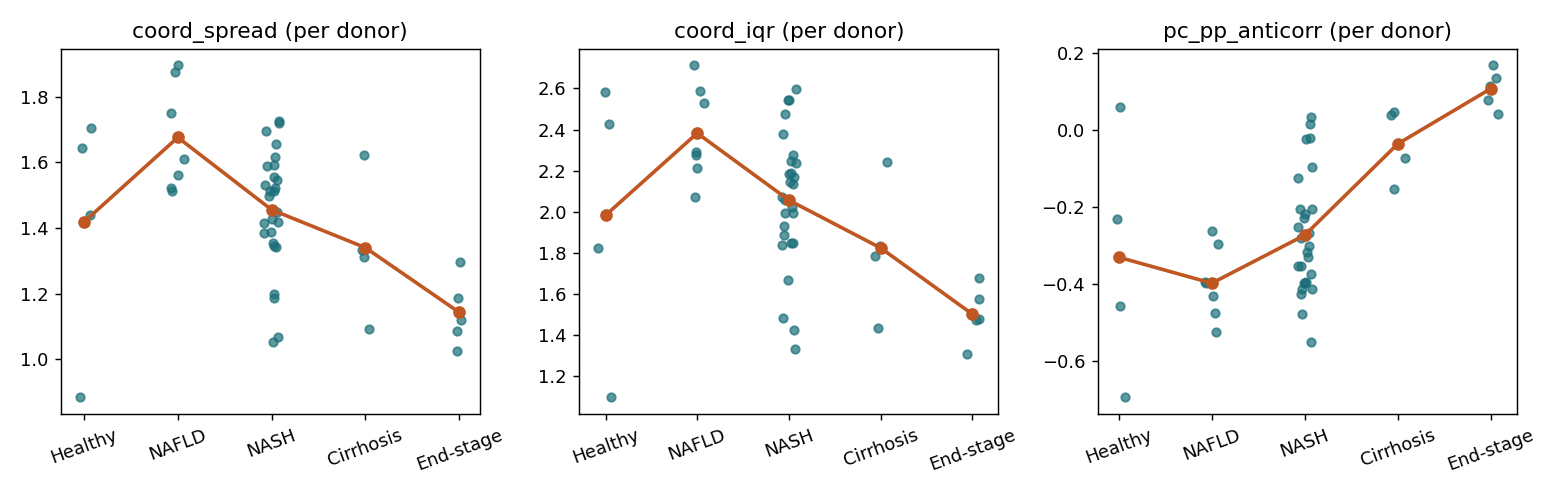
\includegraphics[width=0.92\textwidth]{figures/collapse_unsupervised_lasso.png}\end{center}
\clearpage
\section*{unsupervised\_elasticnet \hfill robustness}
Elastic-net (L1+L2) sparse ruler distilling the Paper-2-trained PCA axis (clean). \textbf{Genes:} 325 PC + 281 PP.
\paragraph{Validation (8-marker healthy gate) \& controls.} Markers correct: 8/8 (PASS). Healthy PC--PP anticorrelation = -0.068 (want strongly negative); split-half reproducibility = +0.689; coherence PC/PP = +0.016/+0.014.
\paragraph{H1 (donor-level collapse, TRANSFER).} coord-spread vs stage rho = -0.492 (perm p = 0.0005); PC--PP anticorr trend rho = +0.483 (perm p = 0.0025).
\paragraph{H2 (zonal slope-loss, held-out).} 606 genes tested; 67\% weaken; median trend rho = -0.121.
\paragraph{H3 (de-zonation $\leftrightarrow$ plasticity, donor-level).} mean rho = -0.020; 21/47 donors $>$0; sign-test p = 0.56.
\begin{center}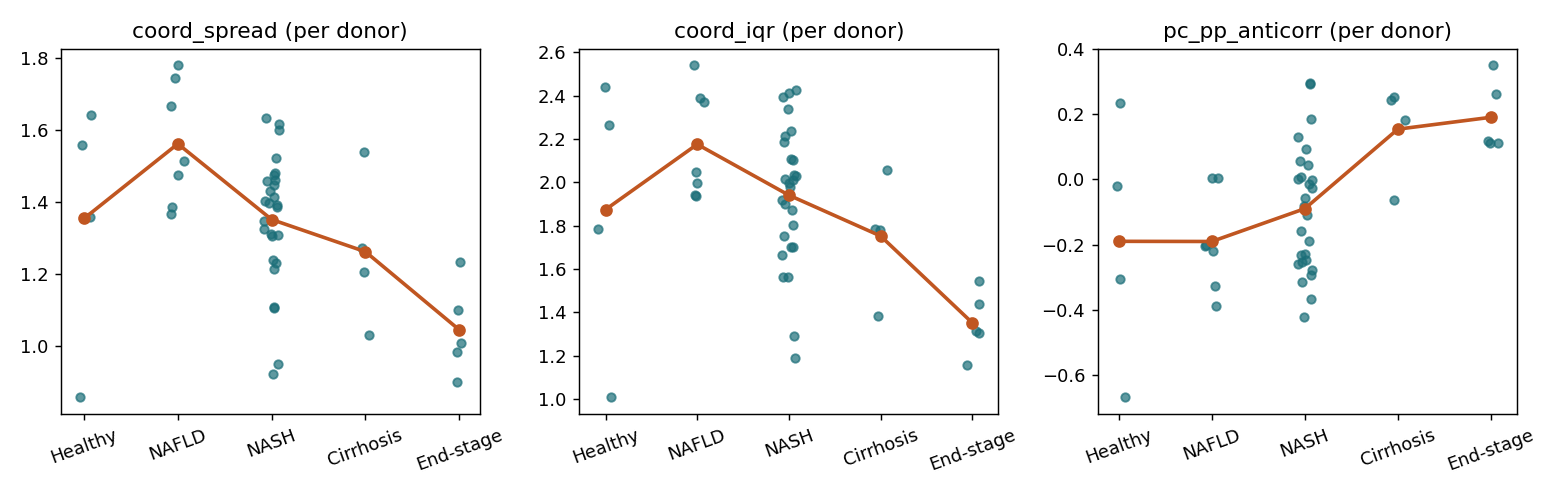
\includegraphics[width=0.92\textwidth]{figures/collapse_unsupervised_elasticnet.png}\end{center}
\clearpage
\section*{paper2\_top250 \hfill exploratory}
Top 250+250 zonated genes by |center-of-mass|. \textbf{Genes:} 250 PC + 250 PP.
\paragraph{Validation (8-marker healthy gate) \& controls.} Markers correct: 8/8 (PASS). Healthy PC--PP anticorrelation = +0.041 (want strongly negative); split-half reproducibility = +0.554; coherence PC/PP = +0.015/+0.011.
\paragraph{H1 (donor-level collapse, TRANSFER).} coord-spread vs stage rho = -0.265 (perm p = 0.067); PC--PP anticorr trend rho = +0.250 (perm p = 0.081).
\paragraph{H2 (zonal slope-loss, held-out).} 483 genes tested; 53\% weaken; median trend rho = -0.011.
\paragraph{H3 (de-zonation $\leftrightarrow$ plasticity, donor-level).} mean rho = +0.006; 26/47 donors $>$0; sign-test p = 0.56.
\begin{center}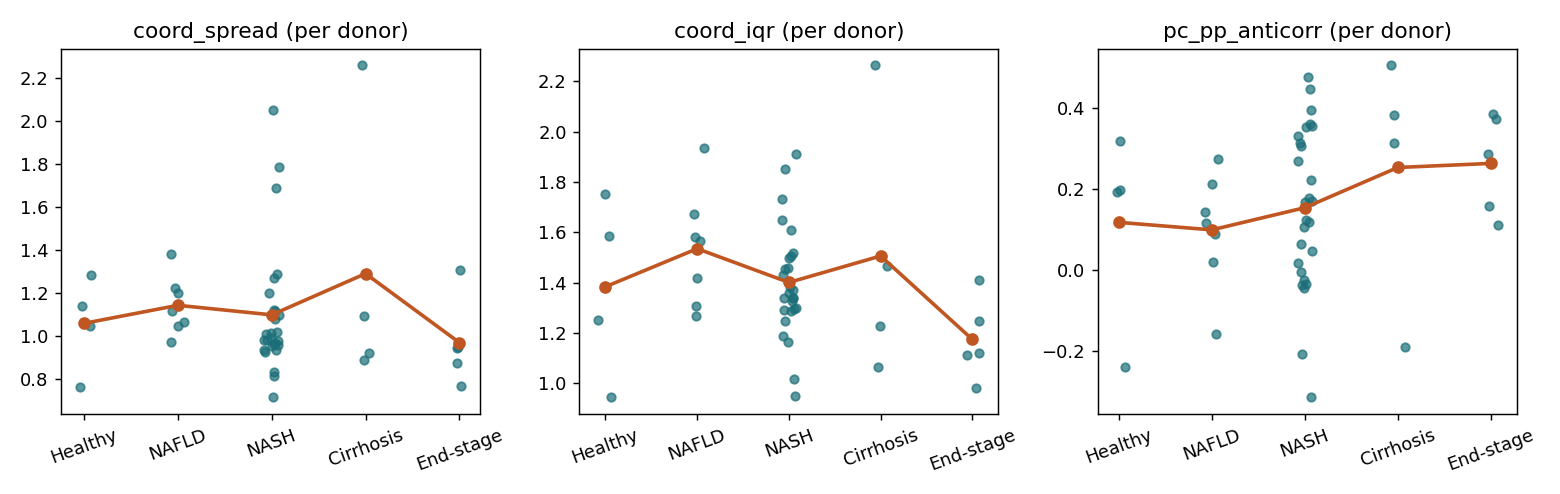
\includegraphics[width=0.92\textwidth]{figures/collapse_paper2_top250.png}\end{center}
\clearpage
\section*{paper2\_full \hfill exploratory}
All significant zonated hepatocyte genes (q<0.05, max-expr>1e-4), split by COM sign (1624+447). \textbf{Genes:} 1624 PC + 447 PP.
\paragraph{Validation (8-marker healthy gate) \& controls.} Markers correct: 8/8 (PASS). Healthy PC--PP anticorrelation = +0.556 (want strongly negative); split-half reproducibility = +0.484; coherence PC/PP = +0.005/+0.009.
\paragraph{H1 (donor-level collapse, TRANSFER).} coord-spread vs stage rho = -0.042 (perm p = 0.77); PC--PP anticorr trend rho = -0.040 (perm p = 0.79).
\paragraph{H2 (zonal slope-loss, held-out).} 2035 genes tested; 41\% weaken; median trend rho = +0.037.
\paragraph{H3 (de-zonation $\leftrightarrow$ plasticity, donor-level).} mean rho = +0.000; 25/47 donors $>$0; sign-test p = 0.77.
\begin{center}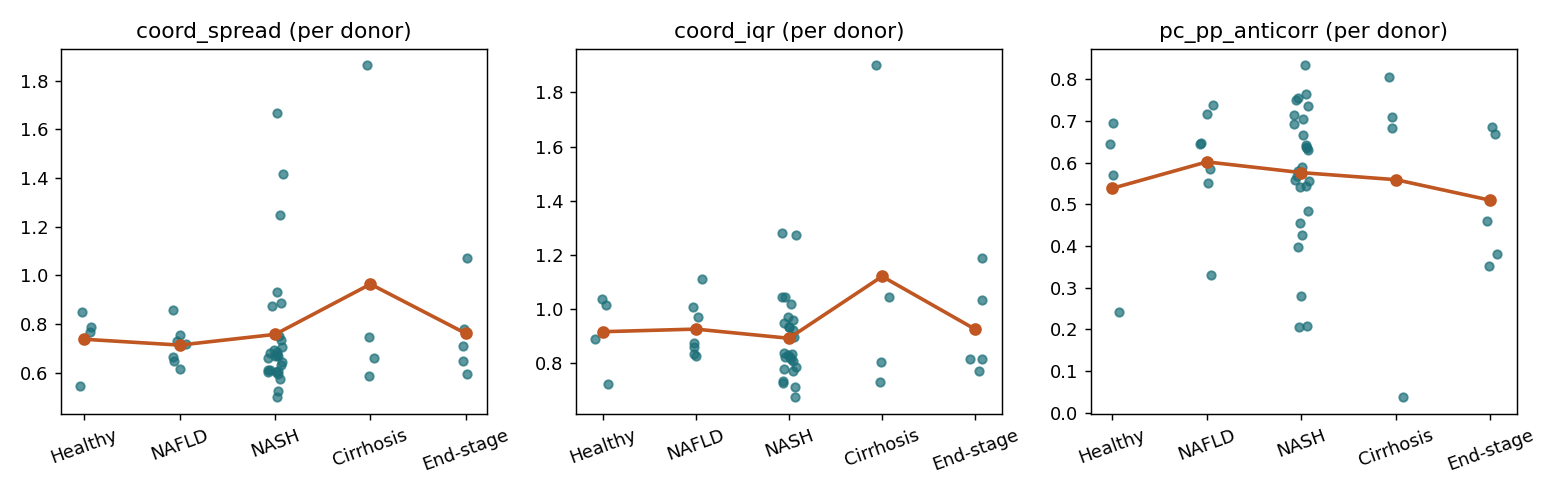
\includegraphics[width=0.92\textwidth]{figures/collapse_paper2_full.png}\end{center}
\clearpage
\section*{full \hfill exploratory}
Legacy transcriptome-wide unweighted signature mean (main pipeline). \textbf{Genes:} 0 PC + 0 PP.
\paragraph{Validation (8-marker healthy gate) \& controls.} Markers correct: 8/8 (PASS). Healthy PC--PP anticorrelation = +0.532 (want strongly negative); split-half reproducibility = +0.464; coherence PC/PP = +0.008/+0.010.
\paragraph{H1 (donor-level collapse, TRANSFER).} coord-spread vs stage rho = +0.021 (perm p = 0.88); PC--PP anticorr trend rho = +0.007 (perm p = 0.97).
\paragraph{H2 (zonal slope-loss, held-out).} 1637 genes tested; 42\% weaken; median trend rho = +0.034.
\paragraph{H3 (de-zonation $\leftrightarrow$ plasticity, donor-level).} mean rho = +0.002; 26/47 donors $>$0; sign-test p = 0.56.
\begin{center}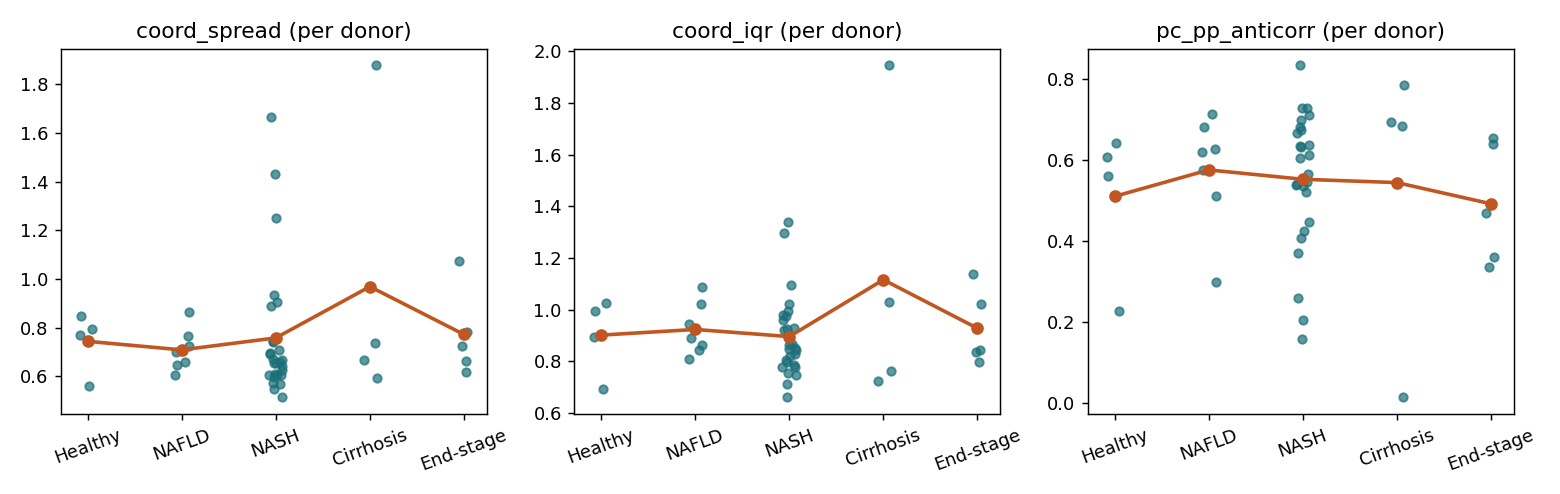
\includegraphics[width=0.92\textwidth]{figures/collapse_full.png}\end{center}
\clearpage
\section*{supervised \hfill exploratory}
Whole-transcriptome multinomial logistic regression trained on Paper 2 zone labels (landmarks excluded). \textbf{Genes:} 4504 PC + 3935 PP.
\paragraph{Validation (8-marker healthy gate) \& controls.} Markers correct: 8/8 (PASS). Healthy PC--PP anticorrelation = -0.005 (want strongly negative); split-half reproducibility = +0.452; coherence PC/PP = +0.064/+0.014.
\paragraph{H1 (donor-level collapse, TRANSFER).} coord-spread vs stage rho = +0.122 (perm p = 0.4); PC--PP anticorr trend rho = +0.569 (perm p = 0.0005).
\paragraph{H2 (zonal slope-loss, held-out).} 100 genes tested; 87\% weaken; median trend rho = -0.169.
\paragraph{H3 (de-zonation $\leftrightarrow$ plasticity, donor-level).} mean rho = +0.003; 27/47 donors $>$0; sign-test p = 0.38.
\begin{center}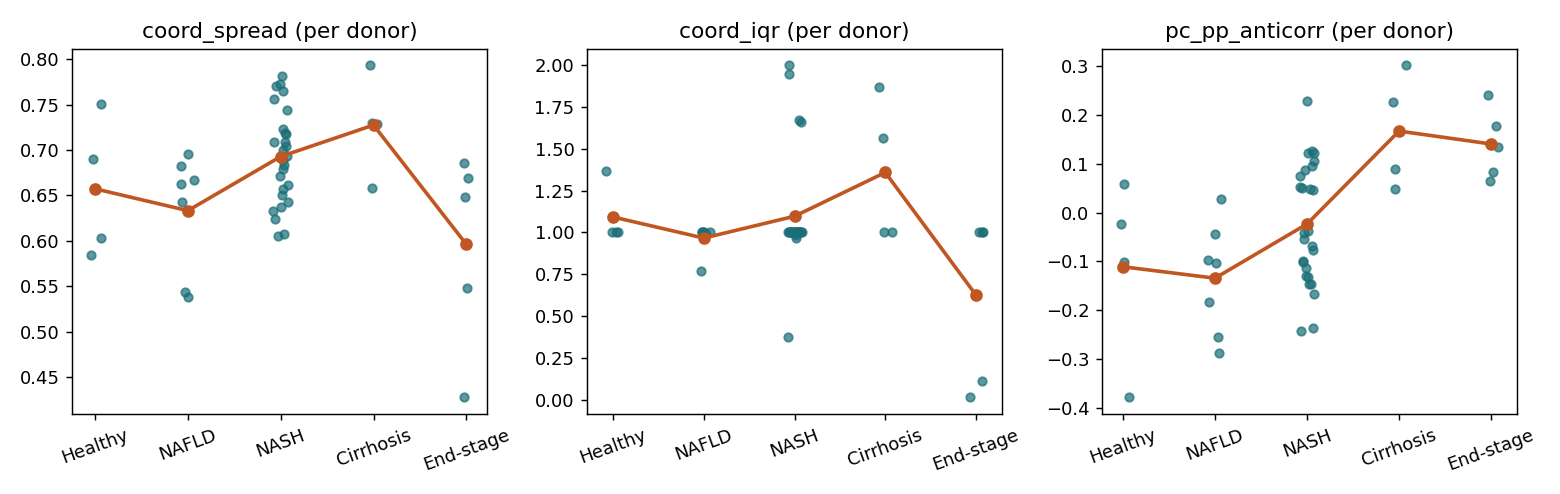
\includegraphics[width=0.92\textwidth]{figures/collapse_supervised.png}\end{center}
\clearpage
\end{document}
